% Options for packages loaded elsewhere
\PassOptionsToPackage{unicode}{hyperref}
\PassOptionsToPackage{hyphens}{url}
\PassOptionsToPackage{dvipsnames,svgnames,x11names}{xcolor}
%
\documentclass[
  letterpaper,
  DIV=11,
  numbers=noendperiod]{scrreprt}

\usepackage{amsmath,amssymb}
\usepackage{lmodern}
\usepackage{iftex}
\ifPDFTeX
  \usepackage[T1]{fontenc}
  \usepackage[utf8]{inputenc}
  \usepackage{textcomp} % provide euro and other symbols
\else % if luatex or xetex
  \usepackage{unicode-math}
  \defaultfontfeatures{Scale=MatchLowercase}
  \defaultfontfeatures[\rmfamily]{Ligatures=TeX,Scale=1}
\fi
% Use upquote if available, for straight quotes in verbatim environments
\IfFileExists{upquote.sty}{\usepackage{upquote}}{}
\IfFileExists{microtype.sty}{% use microtype if available
  \usepackage[]{microtype}
  \UseMicrotypeSet[protrusion]{basicmath} % disable protrusion for tt fonts
}{}
\makeatletter
\@ifundefined{KOMAClassName}{% if non-KOMA class
  \IfFileExists{parskip.sty}{%
    \usepackage{parskip}
  }{% else
    \setlength{\parindent}{0pt}
    \setlength{\parskip}{6pt plus 2pt minus 1pt}}
}{% if KOMA class
  \KOMAoptions{parskip=half}}
\makeatother
\usepackage{xcolor}
\setlength{\emergencystretch}{3em} % prevent overfull lines
\setcounter{secnumdepth}{5}
% Make \paragraph and \subparagraph free-standing
\ifx\paragraph\undefined\else
  \let\oldparagraph\paragraph
  \renewcommand{\paragraph}[1]{\oldparagraph{#1}\mbox{}}
\fi
\ifx\subparagraph\undefined\else
  \let\oldsubparagraph\subparagraph
  \renewcommand{\subparagraph}[1]{\oldsubparagraph{#1}\mbox{}}
\fi

\usepackage{color}
\usepackage{fancyvrb}
\newcommand{\VerbBar}{|}
\newcommand{\VERB}{\Verb[commandchars=\\\{\}]}
\DefineVerbatimEnvironment{Highlighting}{Verbatim}{commandchars=\\\{\}}
% Add ',fontsize=\small' for more characters per line
\usepackage{framed}
\definecolor{shadecolor}{RGB}{241,243,245}
\newenvironment{Shaded}{\begin{snugshade}}{\end{snugshade}}
\newcommand{\AlertTok}[1]{\textcolor[rgb]{0.68,0.00,0.00}{#1}}
\newcommand{\AnnotationTok}[1]{\textcolor[rgb]{0.37,0.37,0.37}{#1}}
\newcommand{\AttributeTok}[1]{\textcolor[rgb]{0.40,0.45,0.13}{#1}}
\newcommand{\BaseNTok}[1]{\textcolor[rgb]{0.68,0.00,0.00}{#1}}
\newcommand{\BuiltInTok}[1]{\textcolor[rgb]{0.00,0.23,0.31}{#1}}
\newcommand{\CharTok}[1]{\textcolor[rgb]{0.13,0.47,0.30}{#1}}
\newcommand{\CommentTok}[1]{\textcolor[rgb]{0.37,0.37,0.37}{#1}}
\newcommand{\CommentVarTok}[1]{\textcolor[rgb]{0.37,0.37,0.37}{\textit{#1}}}
\newcommand{\ConstantTok}[1]{\textcolor[rgb]{0.56,0.35,0.01}{#1}}
\newcommand{\ControlFlowTok}[1]{\textcolor[rgb]{0.00,0.23,0.31}{#1}}
\newcommand{\DataTypeTok}[1]{\textcolor[rgb]{0.68,0.00,0.00}{#1}}
\newcommand{\DecValTok}[1]{\textcolor[rgb]{0.68,0.00,0.00}{#1}}
\newcommand{\DocumentationTok}[1]{\textcolor[rgb]{0.37,0.37,0.37}{\textit{#1}}}
\newcommand{\ErrorTok}[1]{\textcolor[rgb]{0.68,0.00,0.00}{#1}}
\newcommand{\ExtensionTok}[1]{\textcolor[rgb]{0.00,0.23,0.31}{#1}}
\newcommand{\FloatTok}[1]{\textcolor[rgb]{0.68,0.00,0.00}{#1}}
\newcommand{\FunctionTok}[1]{\textcolor[rgb]{0.28,0.35,0.67}{#1}}
\newcommand{\ImportTok}[1]{\textcolor[rgb]{0.00,0.46,0.62}{#1}}
\newcommand{\InformationTok}[1]{\textcolor[rgb]{0.37,0.37,0.37}{#1}}
\newcommand{\KeywordTok}[1]{\textcolor[rgb]{0.00,0.23,0.31}{#1}}
\newcommand{\NormalTok}[1]{\textcolor[rgb]{0.00,0.23,0.31}{#1}}
\newcommand{\OperatorTok}[1]{\textcolor[rgb]{0.37,0.37,0.37}{#1}}
\newcommand{\OtherTok}[1]{\textcolor[rgb]{0.00,0.23,0.31}{#1}}
\newcommand{\PreprocessorTok}[1]{\textcolor[rgb]{0.68,0.00,0.00}{#1}}
\newcommand{\RegionMarkerTok}[1]{\textcolor[rgb]{0.00,0.23,0.31}{#1}}
\newcommand{\SpecialCharTok}[1]{\textcolor[rgb]{0.37,0.37,0.37}{#1}}
\newcommand{\SpecialStringTok}[1]{\textcolor[rgb]{0.13,0.47,0.30}{#1}}
\newcommand{\StringTok}[1]{\textcolor[rgb]{0.13,0.47,0.30}{#1}}
\newcommand{\VariableTok}[1]{\textcolor[rgb]{0.07,0.07,0.07}{#1}}
\newcommand{\VerbatimStringTok}[1]{\textcolor[rgb]{0.13,0.47,0.30}{#1}}
\newcommand{\WarningTok}[1]{\textcolor[rgb]{0.37,0.37,0.37}{\textit{#1}}}

\providecommand{\tightlist}{%
  \setlength{\itemsep}{0pt}\setlength{\parskip}{0pt}}\usepackage{longtable,booktabs,array}
\usepackage{calc} % for calculating minipage widths
% Correct order of tables after \paragraph or \subparagraph
\usepackage{etoolbox}
\makeatletter
\patchcmd\longtable{\par}{\if@noskipsec\mbox{}\fi\par}{}{}
\makeatother
% Allow footnotes in longtable head/foot
\IfFileExists{footnotehyper.sty}{\usepackage{footnotehyper}}{\usepackage{footnote}}
\makesavenoteenv{longtable}
\usepackage{graphicx}
\makeatletter
\def\maxwidth{\ifdim\Gin@nat@width>\linewidth\linewidth\else\Gin@nat@width\fi}
\def\maxheight{\ifdim\Gin@nat@height>\textheight\textheight\else\Gin@nat@height\fi}
\makeatother
% Scale images if necessary, so that they will not overflow the page
% margins by default, and it is still possible to overwrite the defaults
% using explicit options in \includegraphics[width, height, ...]{}
\setkeys{Gin}{width=\maxwidth,height=\maxheight,keepaspectratio}
% Set default figure placement to htbp
\makeatletter
\def\fps@figure{htbp}
\makeatother

\KOMAoption{captions}{tableheading}
\makeatletter
\makeatother
\makeatletter
\@ifpackageloaded{bookmark}{}{\usepackage{bookmark}}
\makeatother
\makeatletter
\@ifpackageloaded{caption}{}{\usepackage{caption}}
\AtBeginDocument{%
\ifdefined\contentsname
  \renewcommand*\contentsname{Table of contents}
\else
  \newcommand\contentsname{Table of contents}
\fi
\ifdefined\listfigurename
  \renewcommand*\listfigurename{List of Figures}
\else
  \newcommand\listfigurename{List of Figures}
\fi
\ifdefined\listtablename
  \renewcommand*\listtablename{List of Tables}
\else
  \newcommand\listtablename{List of Tables}
\fi
\ifdefined\figurename
  \renewcommand*\figurename{Figure}
\else
  \newcommand\figurename{Figure}
\fi
\ifdefined\tablename
  \renewcommand*\tablename{Table}
\else
  \newcommand\tablename{Table}
\fi
}
\@ifpackageloaded{float}{}{\usepackage{float}}
\floatstyle{ruled}
\@ifundefined{c@chapter}{\newfloat{codelisting}{h}{lop}}{\newfloat{codelisting}{h}{lop}[chapter]}
\floatname{codelisting}{Listing}
\newcommand*\listoflistings{\listof{codelisting}{List of Listings}}
\makeatother
\makeatletter
\@ifpackageloaded{caption}{}{\usepackage{caption}}
\@ifpackageloaded{subcaption}{}{\usepackage{subcaption}}
\makeatother
\makeatletter
\@ifpackageloaded{tcolorbox}{}{\usepackage[many]{tcolorbox}}
\makeatother
\makeatletter
\@ifundefined{shadecolor}{\definecolor{shadecolor}{rgb}{.97, .97, .97}}
\makeatother
\makeatletter
\makeatother
\ifLuaTeX
  \usepackage{selnolig}  % disable illegal ligatures
\fi
\IfFileExists{bookmark.sty}{\usepackage{bookmark}}{\usepackage{hyperref}}
\IfFileExists{xurl.sty}{\usepackage{xurl}}{} % add URL line breaks if available
\urlstyle{same} % disable monospaced font for URLs
\hypersetup{
  pdftitle={Ali Gokmen / Peace \& Trust Progress Journal},
  colorlinks=true,
  linkcolor={blue},
  filecolor={Maroon},
  citecolor={Blue},
  urlcolor={Blue},
  pdfcreator={LaTeX via pandoc}}

\title{Ali Gokmen / Peace \& Trust Progress Journal}
\author{}
\date{}

\begin{document}
\maketitle
\ifdefined\Shaded\renewenvironment{Shaded}{\begin{tcolorbox}[boxrule=0pt, frame hidden, breakable, borderline west={3pt}{0pt}{shadecolor}, sharp corners, enhanced, interior hidden]}{\end{tcolorbox}}\fi

\renewcommand*\contentsname{Table of contents}
{
\hypersetup{linkcolor=}
\setcounter{tocdepth}{2}
\tableofcontents
}
\bookmarksetup{startatroot}

\hypertarget{introduction}{%
\chapter*{Introduction}\label{introduction}}
\addcontentsline{toc}{chapter}{Introduction}

This progress journal covers {[}STUDENT NAME SURNAME / PROJECT GROUP
NAME{]}'s work during their term at
\href{https://mef-bda503.github.io/fall22/}{BDA 503 Fall 2022}.

Each section is an assignment or an individual work.

\bookmarksetup{startatroot}

\hypertarget{assignment-1}{%
\chapter{Assignment 1}\label{assignment-1}}

Ali Gökmen\\
2022-10-16

\hfill\break

Hello, I am Muhammed Ali Gökmen and 24 yo. I finished my Bachelor of
City and Regional Planning in 2020 from Mimar Sinan Fine Arts University
with the thesis of ``The Relationship Between Smart Cities and Smart
Energy Systems: The sample of Urban Planning''. I examined in one part
of my thesis that how smart energy systems can effectively manage by
technology of big data and IoT. Also in my university years, I always
curious about data and how to process it effectively. I have got Python
class in university, some data analytics and statistics courses on Udemy
and other educational places to get some insights and see what I can do
in this area on the basis of personal curiosity. Besides, in my part
time job I had the chance to practice the theoretical knowledge I
learned from this course. While last year of my university I worked for
Turkish Airlines as a part time clerk. I enhanced my data analytics
skills in this meantime to have a oppurtunity to get hired there and
keep pushing developing myself. After graduation I got hired as a
specialist in the Management of Strategic Planning and Data Analysis
Turkish Airlines and still working there now. In general, we are
responsible for the analysis of reports flowing into our database.
Basically, we clean the data by doing the relevant filters, then analyze
it and focus on making meaningful inferences. We report the results to
our executives in order to contribute to their decision-making
processes.I want to use data analytics skills in our monthly sales
forecasting process to shape it more understandable and realistic.

\href{https://www.linkedin.com/in/maligokmen/}{\textbf{\emph{Here is my
linkedin profile}}}

\hypertarget{dashboard-builder-building-shiny-apps-without-writing-any-code}{%
\section{\texorpdfstring{\textbf{Dashboard-Builder: Building Shiny Apps
without writing any
code}}{Dashboard-Builder: Building Shiny Apps without writing any code}}\label{dashboard-builder-building-shiny-apps-without-writing-any-code}}

I have preferred to watch the conference named ``Dashboard-Builder:
Building Shiny Apps'' presenting by Peter Gandenberger.

In this conference, Mr.~Ganderberger appealed to people who want to make
dashboard but don't know how to code in R and consider that R complex.
So, last project of Peter's team allows people to make interactive
dashboards.

This drag\&drop dashboard builder lowering the barrier for entry new
users starting their data-science journey.

Main steps:

\begin{enumerate}
\def\labelenumi{\arabic{enumi}.}
\tightlist
\item
  Import data
\item
  Build Dashboard
\item
  Export
\item
  Improve \& Extend
\end{enumerate}

Here is a screenshot of an example dashboard:

\hypertarget{r-posts-relevant-to-my-interest}{%
\section{3 R Posts relevant to my
interest}\label{r-posts-relevant-to-my-interest}}

\hypertarget{dot-chart}{%
\subsection{Dot Chart}\label{dot-chart}}

\begin{Shaded}
\begin{Highlighting}[]
\DocumentationTok{\#\#\# Dot Chart}

\DocumentationTok{\#\#\# Setting seed for reproducibility}
\FunctionTok{set.seed}\NormalTok{(}\DecValTok{1}\NormalTok{)}

\DocumentationTok{\#\#\# Defining variables}
\NormalTok{month }\OtherTok{\textless{}{-}}\NormalTok{ month.name}
\NormalTok{expected }\OtherTok{\textless{}{-}} \FunctionTok{c}\NormalTok{(}\DecValTok{15}\NormalTok{, }\DecValTok{16}\NormalTok{, }\DecValTok{20}\NormalTok{, }\DecValTok{31}\NormalTok{, }\DecValTok{11}\NormalTok{, }\DecValTok{6}\NormalTok{,}
              \DecValTok{17}\NormalTok{, }\DecValTok{22}\NormalTok{, }\DecValTok{32}\NormalTok{, }\DecValTok{12}\NormalTok{, }\DecValTok{19}\NormalTok{, }\DecValTok{20}\NormalTok{)}
\NormalTok{sold }\OtherTok{\textless{}{-}} \FunctionTok{c}\NormalTok{(}\DecValTok{8}\NormalTok{, }\DecValTok{18}\NormalTok{, }\DecValTok{12}\NormalTok{, }\DecValTok{10}\NormalTok{, }\DecValTok{41}\NormalTok{, }\DecValTok{2}\NormalTok{,}
          \DecValTok{19}\NormalTok{, }\DecValTok{26}\NormalTok{, }\DecValTok{14}\NormalTok{, }\DecValTok{16}\NormalTok{, }\DecValTok{9}\NormalTok{, }\DecValTok{13}\NormalTok{)}
\NormalTok{quarter }\OtherTok{\textless{}{-}} \FunctionTok{c}\NormalTok{(}\FunctionTok{rep}\NormalTok{(}\DecValTok{1}\NormalTok{, }\DecValTok{3}\NormalTok{), }\FunctionTok{rep}\NormalTok{(}\DecValTok{2}\NormalTok{, }\DecValTok{3}\NormalTok{), }\FunctionTok{rep}\NormalTok{(}\DecValTok{3}\NormalTok{, }\DecValTok{3}\NormalTok{), }\FunctionTok{rep}\NormalTok{(}\DecValTok{4}\NormalTok{, }\DecValTok{3}\NormalTok{))}

\DocumentationTok{\#\#\# Printing data}
\NormalTok{data }\OtherTok{\textless{}{-}} \FunctionTok{data.frame}\NormalTok{(month, expected, sold, quarter)}
\NormalTok{data}
\end{Highlighting}
\end{Shaded}

\begin{verbatim}
       month expected sold quarter
1    January       15    8       1
2   February       16   18       1
3      March       20   12       1
4      April       31   10       2
5        May       11   41       2
6       June        6    2       2
7       July       17   19       3
8     August       22   26       3
9  September       32   14       3
10   October       12   16       4
11  November       19    9       4
12  December       20   13       4
\end{verbatim}

\begin{Shaded}
\begin{Highlighting}[]
\DocumentationTok{\#\#\# Chart}
\FunctionTok{dotchart}\NormalTok{(data}\SpecialCharTok{$}\NormalTok{sold, }\AttributeTok{labels =}\NormalTok{ data}\SpecialCharTok{$}\NormalTok{month, }\AttributeTok{pch =} \DecValTok{21}\NormalTok{, }\AttributeTok{bg =} \StringTok{"green"}\NormalTok{, }\AttributeTok{pt.cex =} \FloatTok{1.5}\NormalTok{)}
\end{Highlighting}
\end{Shaded}

\begin{figure}[H]

{\centering 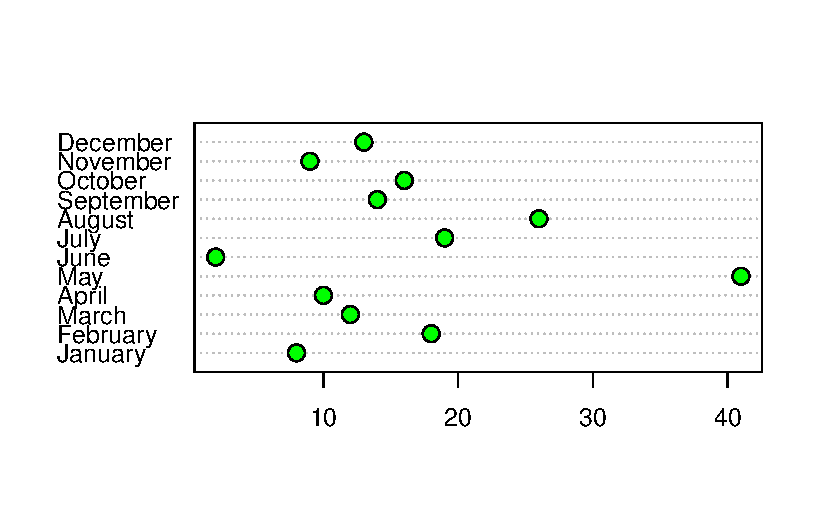
\includegraphics{./assignment1_files/figure-pdf/unnamed-chunk-1-1.pdf}

}

\end{figure}

\hypertarget{bar-plot-chart}{%
\subsection{Bar Plot Chart}\label{bar-plot-chart}}

Bar plot charts can be used efficiently for:

-to analyze a comparative study between various categories

-to analyze the change of a variable over time in months or years

For example:

\begin{Shaded}
\begin{Highlighting}[]
\FunctionTok{barplot}\NormalTok{(airquality}\SpecialCharTok{$}\NormalTok{Ozone, }\AttributeTok{main =} \StringTok{\textquotesingle{}Ozone Concenteration in air\textquotesingle{}}\NormalTok{, }
        \AttributeTok{xlab =} \StringTok{\textquotesingle{}ozone levels\textquotesingle{}}\NormalTok{, }\AttributeTok{col =}\StringTok{\textquotesingle{}blue\textquotesingle{}}\NormalTok{, }\AttributeTok{horiz =} \ConstantTok{FALSE}\NormalTok{)}
\end{Highlighting}
\end{Shaded}

\begin{figure}[H]

{\centering 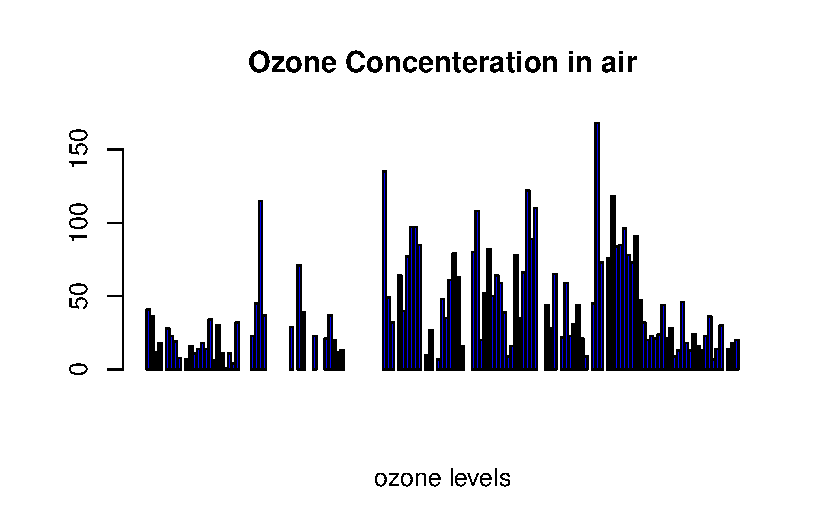
\includegraphics{./assignment1_files/figure-pdf/unnamed-chunk-2-1.pdf}

}

\end{figure}

\hypertarget{density-plot-chart}{%
\subsection{Density Plot Chart}\label{density-plot-chart}}

Density plot chart can be used when we need to see representation of the
distribution of a variable.

For example:

\begin{Shaded}
\begin{Highlighting}[]
\FunctionTok{library}\NormalTok{(ggplot2)}
\FunctionTok{theme\_set}\NormalTok{(}\FunctionTok{theme\_classic}\NormalTok{())}

\CommentTok{\# Plot}
\NormalTok{g }\OtherTok{\textless{}{-}} \FunctionTok{ggplot}\NormalTok{(mpg, }\FunctionTok{aes}\NormalTok{(cty))}
\NormalTok{g }\SpecialCharTok{+} \FunctionTok{geom\_density}\NormalTok{(}\FunctionTok{aes}\NormalTok{(}\AttributeTok{fill=}\FunctionTok{factor}\NormalTok{(cyl)), }\AttributeTok{alpha=}\FloatTok{0.8}\NormalTok{) }\SpecialCharTok{+} 
    \FunctionTok{labs}\NormalTok{(}\AttributeTok{title=}\StringTok{"Density plot"}\NormalTok{, }
         \AttributeTok{subtitle=}\StringTok{"City Mileage Grouped by Number of cylinders"}\NormalTok{,}
         \AttributeTok{caption=}\StringTok{"Source: mpg"}\NormalTok{,}
         \AttributeTok{x=}\StringTok{"City Mileage"}\NormalTok{,}
         \AttributeTok{fill=}\StringTok{"\# Cylinders"}\NormalTok{)}
\end{Highlighting}
\end{Shaded}

\begin{figure}[H]

{\centering 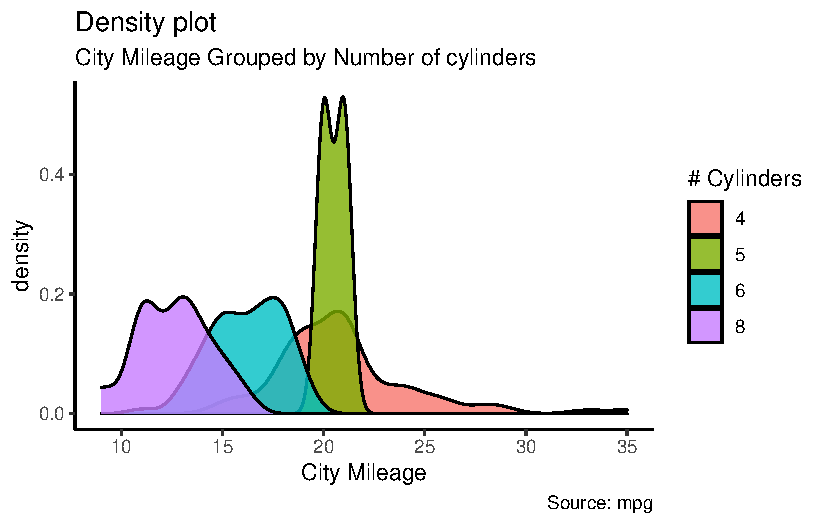
\includegraphics{./assignment1_files/figure-pdf/unnamed-chunk-3-1.pdf}

}

\end{figure}

\href{https://www.geeksforgeeks.org/}{\textbf{Source Link}}



\end{document}
